\documentclass[border=5pt]{standalone}
%%%<
\usepackage{verbatim}
%%%>
\usepackage{pgfplots}
\pgfplotsset{width=7cm,compat=1.8}
\begin{comment}
:Title: Plot with error intervals
:Tags: 2D;Stacked plots
:Author: Jake
:Slug: error-intervals

Here, the trick is to use stack plots=y together with \closedcycle
to create the error bands.

We define a new command,
\addplotwitherrorbands[<optional styles>]{<function>}{<positive error>}
{<negative error>} for this spurpose.

This code was written by Jake on TeX.SE.
\end{comment}
\tikzset{
    error band/.style={fill=orange},
    error band style/.style={
        error band/.append style=#1
    }
}
\newcommand{\addplotwitherrorband}[4][]{
  \addplot [#1, draw=none, stack plots=y, forget plot] {#2-(#3)};
  \addplot +[#1, draw=none, stack plots=y, error band] {(#3)+(#4)}\closedcycle;
  \addplot [#1, draw=none, stack plots=y, forget plot] {-(#2)-(#3)};
  \addplot [#1, forget plot] {#2};
}
\begin{document}
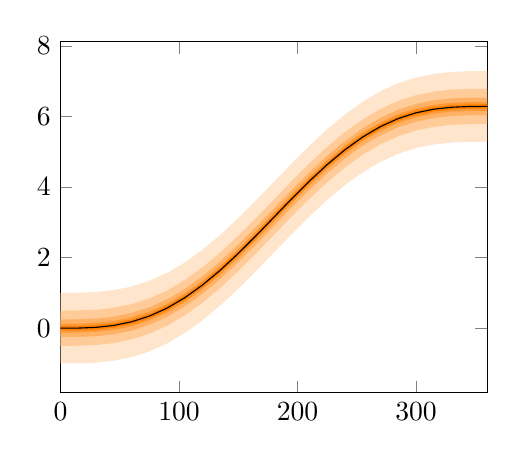
\begin{tikzpicture}[
    declare function={f(\x)=rad(\x)-sin(\x);}
  ]
  \begin{axis}[domain = 0:360, enlarge x limits = false,
      cycle list = {
        error band style = orange!20\\
        error band style = orange!40\\
        error band style = orange!60\\
        error band style = orange!80\\
        error band style = orange!100\\
      }
    ]
    \pgfplotsinvokeforeach{1,0.5,0.25,0.125, 0.0625} {
      \addplotwitherrorband [] {f(x)}{#1}{#1}
    }
  \end{axis}
\end{tikzpicture}
\end{document}
